\documentclass[tikz, border=10pt]{standalone}
\usepackage{pgfplots}
\usepackage{amsmath}
\usetikzlibrary{backgrounds}
\pgfplotsset{compat=1.18}

\begin{document}
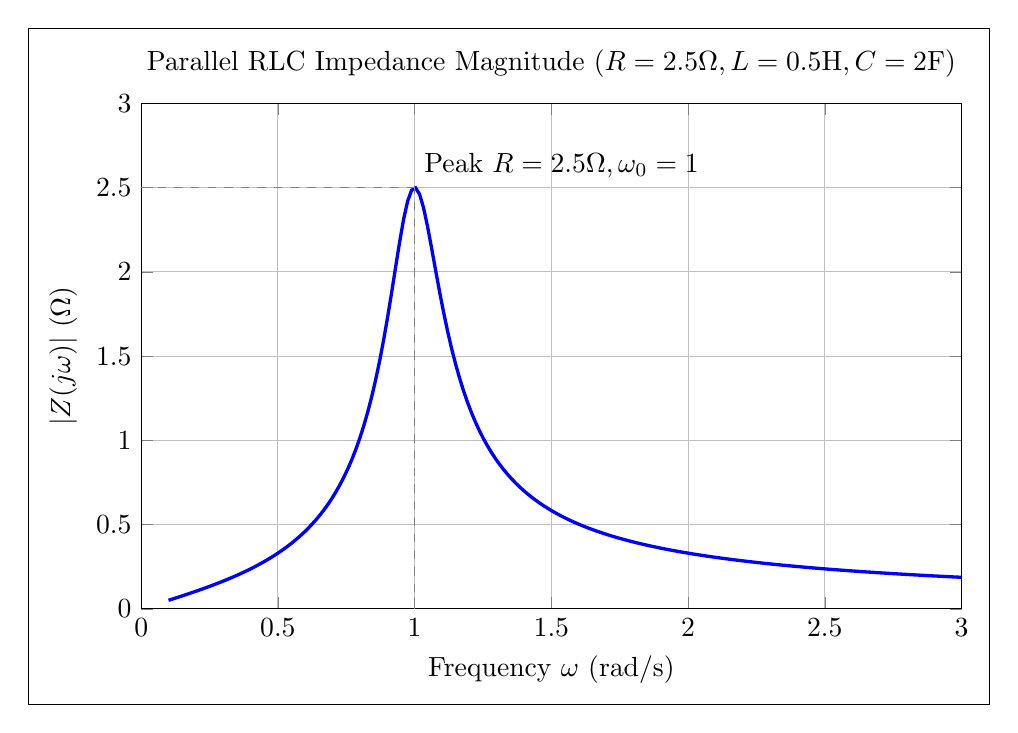
\begin{tikzpicture}[show background rectangle]
    \begin{axis}[
        width=12cm, height=8cm,
        title={Parallel RLC Impedance Magnitude ($R=2.5\Omega, L=0.5\text{H}, C=2\text{F}$)},
        xlabel={Frequency $\omega$ (rad/s)},
        ylabel={$|Z(j\omega)|$ ($\Omega$)},
        grid=both,
        xmin=0, xmax=3,
        ymin=0, ymax=3,
        minor grid style={gray!25},
        major grid style={gray!50},
        domain=0.1:3,
        samples=200,
    ]

    % |Z| = 1 / sqrt( (1/R)^2 + (wC - 1/wL)^2 )
    % |Z| = 1 / sqrt( (1/2.5)^2 + (2x - 1/(0.5x))^2 )
    \addplot[blue, very thick] { 1 / sqrt( (1/2.5)^2 + (2*x - 2/x)^2 ) };
    
    % Markers for peak
    \draw[dashed, gray] (axis cs:1, 0) -- (axis cs:1, 2.5);
    \draw[dashed, gray] (axis cs:0, 2.5) -- (axis cs:1, 2.5);
    \node[anchor=south west] at (axis cs:1, 2.5) {Peak $R=2.5\Omega, \omega_0=1$};

    \end{axis}
\end{tikzpicture}
\end{document}
